% Options for packages loaded elsewhere
\PassOptionsToPackage{unicode}{hyperref}
\PassOptionsToPackage{hyphens}{url}
%
\documentclass[
]{article}
\usepackage{amsmath,amssymb}
\usepackage{iftex}
\ifPDFTeX
  \usepackage[T1]{fontenc}
  \usepackage[utf8]{inputenc}
  \usepackage{textcomp} % provide euro and other symbols
\else % if luatex or xetex
  \usepackage{unicode-math} % this also loads fontspec
  \defaultfontfeatures{Scale=MatchLowercase}
  \defaultfontfeatures[\rmfamily]{Ligatures=TeX,Scale=1}
\fi
\usepackage{lmodern}
\ifPDFTeX\else
  % xetex/luatex font selection
\fi
% Use upquote if available, for straight quotes in verbatim environments
\IfFileExists{upquote.sty}{\usepackage{upquote}}{}
\IfFileExists{microtype.sty}{% use microtype if available
  \usepackage[]{microtype}
  \UseMicrotypeSet[protrusion]{basicmath} % disable protrusion for tt fonts
}{}
\makeatletter
\@ifundefined{KOMAClassName}{% if non-KOMA class
  \IfFileExists{parskip.sty}{%
    \usepackage{parskip}
  }{% else
    \setlength{\parindent}{0pt}
    \setlength{\parskip}{6pt plus 2pt minus 1pt}}
}{% if KOMA class
  \KOMAoptions{parskip=half}}
\makeatother
\usepackage{xcolor}
\usepackage[margin=1in]{geometry}
\usepackage{color}
\usepackage{fancyvrb}
\newcommand{\VerbBar}{|}
\newcommand{\VERB}{\Verb[commandchars=\\\{\}]}
\DefineVerbatimEnvironment{Highlighting}{Verbatim}{commandchars=\\\{\}}
% Add ',fontsize=\small' for more characters per line
\usepackage{framed}
\definecolor{shadecolor}{RGB}{248,248,248}
\newenvironment{Shaded}{\begin{snugshade}}{\end{snugshade}}
\newcommand{\AlertTok}[1]{\textcolor[rgb]{0.94,0.16,0.16}{#1}}
\newcommand{\AnnotationTok}[1]{\textcolor[rgb]{0.56,0.35,0.01}{\textbf{\textit{#1}}}}
\newcommand{\AttributeTok}[1]{\textcolor[rgb]{0.13,0.29,0.53}{#1}}
\newcommand{\BaseNTok}[1]{\textcolor[rgb]{0.00,0.00,0.81}{#1}}
\newcommand{\BuiltInTok}[1]{#1}
\newcommand{\CharTok}[1]{\textcolor[rgb]{0.31,0.60,0.02}{#1}}
\newcommand{\CommentTok}[1]{\textcolor[rgb]{0.56,0.35,0.01}{\textit{#1}}}
\newcommand{\CommentVarTok}[1]{\textcolor[rgb]{0.56,0.35,0.01}{\textbf{\textit{#1}}}}
\newcommand{\ConstantTok}[1]{\textcolor[rgb]{0.56,0.35,0.01}{#1}}
\newcommand{\ControlFlowTok}[1]{\textcolor[rgb]{0.13,0.29,0.53}{\textbf{#1}}}
\newcommand{\DataTypeTok}[1]{\textcolor[rgb]{0.13,0.29,0.53}{#1}}
\newcommand{\DecValTok}[1]{\textcolor[rgb]{0.00,0.00,0.81}{#1}}
\newcommand{\DocumentationTok}[1]{\textcolor[rgb]{0.56,0.35,0.01}{\textbf{\textit{#1}}}}
\newcommand{\ErrorTok}[1]{\textcolor[rgb]{0.64,0.00,0.00}{\textbf{#1}}}
\newcommand{\ExtensionTok}[1]{#1}
\newcommand{\FloatTok}[1]{\textcolor[rgb]{0.00,0.00,0.81}{#1}}
\newcommand{\FunctionTok}[1]{\textcolor[rgb]{0.13,0.29,0.53}{\textbf{#1}}}
\newcommand{\ImportTok}[1]{#1}
\newcommand{\InformationTok}[1]{\textcolor[rgb]{0.56,0.35,0.01}{\textbf{\textit{#1}}}}
\newcommand{\KeywordTok}[1]{\textcolor[rgb]{0.13,0.29,0.53}{\textbf{#1}}}
\newcommand{\NormalTok}[1]{#1}
\newcommand{\OperatorTok}[1]{\textcolor[rgb]{0.81,0.36,0.00}{\textbf{#1}}}
\newcommand{\OtherTok}[1]{\textcolor[rgb]{0.56,0.35,0.01}{#1}}
\newcommand{\PreprocessorTok}[1]{\textcolor[rgb]{0.56,0.35,0.01}{\textit{#1}}}
\newcommand{\RegionMarkerTok}[1]{#1}
\newcommand{\SpecialCharTok}[1]{\textcolor[rgb]{0.81,0.36,0.00}{\textbf{#1}}}
\newcommand{\SpecialStringTok}[1]{\textcolor[rgb]{0.31,0.60,0.02}{#1}}
\newcommand{\StringTok}[1]{\textcolor[rgb]{0.31,0.60,0.02}{#1}}
\newcommand{\VariableTok}[1]{\textcolor[rgb]{0.00,0.00,0.00}{#1}}
\newcommand{\VerbatimStringTok}[1]{\textcolor[rgb]{0.31,0.60,0.02}{#1}}
\newcommand{\WarningTok}[1]{\textcolor[rgb]{0.56,0.35,0.01}{\textbf{\textit{#1}}}}
\usepackage{longtable,booktabs,array}
\usepackage{calc} % for calculating minipage widths
% Correct order of tables after \paragraph or \subparagraph
\usepackage{etoolbox}
\makeatletter
\patchcmd\longtable{\par}{\if@noskipsec\mbox{}\fi\par}{}{}
\makeatother
% Allow footnotes in longtable head/foot
\IfFileExists{footnotehyper.sty}{\usepackage{footnotehyper}}{\usepackage{footnote}}
\makesavenoteenv{longtable}
\usepackage{graphicx}
\makeatletter
\def\maxwidth{\ifdim\Gin@nat@width>\linewidth\linewidth\else\Gin@nat@width\fi}
\def\maxheight{\ifdim\Gin@nat@height>\textheight\textheight\else\Gin@nat@height\fi}
\makeatother
% Scale images if necessary, so that they will not overflow the page
% margins by default, and it is still possible to overwrite the defaults
% using explicit options in \includegraphics[width, height, ...]{}
\setkeys{Gin}{width=\maxwidth,height=\maxheight,keepaspectratio}
% Set default figure placement to htbp
\makeatletter
\def\fps@figure{htbp}
\makeatother
\setlength{\emergencystretch}{3em} % prevent overfull lines
\providecommand{\tightlist}{%
  \setlength{\itemsep}{0pt}\setlength{\parskip}{0pt}}
\setcounter{secnumdepth}{-\maxdimen} % remove section numbering
\ifLuaTeX
  \usepackage{selnolig}  % disable illegal ligatures
\fi
\usepackage{bookmark}
\IfFileExists{xurl.sty}{\usepackage{xurl}}{} % add URL line breaks if available
\urlstyle{same}
\hypersetup{
  pdftitle={The N400 effect when singular gendered antecedents are co-indexed with (a) himself or herself (b) themselves},
  pdfauthor={Joanna Morris},
  hidelinks,
  pdfcreator={LaTeX via pandoc}}

\title{The N400 effect when singular gendered antecedents are co-indexed
with (a) \emph{himself} or \emph{herself} (b) \emph{themselves}}
\author{Joanna Morris}
\date{2024-08-19}

\begin{document}
\maketitle

\subsection{Overview}\label{overview}

This document contains the code to reproduce the statistical analyses
described in {[}Prasad and Morris (2024){]}

This document has two sections:

\begin{enumerate}
\def\labelenumi{\arabic{enumi}.}
\setcounter{enumi}{1}
\tightlist
\item
  \hyperref[gender]{Analysis 1: The N400 effect when antecedents are
  co-indexed with \emph{himself} or \emph{herself}}
\item
  \hyperref[number]{Analysis 2: The N400 effect when antecedents are
  co-indexed with \emph{themselves}}
\end{enumerate}

\subsection{Define functions, set parameters and
load}\label{define-functions-set-parameters-and-load}

Define standard error of mean function

\begin{Shaded}
\begin{Highlighting}[]
\NormalTok{sem }\OtherTok{\textless{}{-}} \ControlFlowTok{function}\NormalTok{(x) }\FunctionTok{sd}\NormalTok{(x)}\SpecialCharTok{/}\FunctionTok{sqrt}\NormalTok{(}\FunctionTok{length}\NormalTok{(x))}
\end{Highlighting}
\end{Shaded}

Before we begin, let's set some general parameters for \texttt{ggplot2}.
We will set a general theme using the \texttt{theme\_set()} function. We
will use the `classic' theme which gives us clean white background
rather than the default grey with white grid lines. And we will position
the legend at the top of the graph rather than at the right side which
is the default.

\subsection{Load the data}\label{load-the-data}

Then we re-order factor levels for \emph{Anteriority} \&
\emph{Referentiality}

\begin{verbatim}
## [1] "Frontal"        "FrontoCentral"  "Central"        "CentroParietal"
## [5] "Parietal"
\end{verbatim}

\begin{verbatim}
## [1] "Referential"    "NonReferential"
\end{verbatim}

\begin{verbatim}
## [1] "Frontal"        "FrontoCentral"  "Central"        "CentroParietal"
## [5] "Parietal"
\end{verbatim}

\begin{verbatim}
## [1] "Referential"    "NonReferential"
\end{verbatim}

\subsection{Check ANOVA assumptions}\label{check-anova-assumptions}

\begin{itemize}
\tightlist
\item
  \emph{No significant outliers in any cell of the design}. This can be
  checked by visualizing the data using box plot methods and by using
  the function \texttt{identify\_outliers()} in the \texttt{rstatix}
  package.
\end{itemize}

\begin{longtable}[]{@{}
  >{\raggedleft\arraybackslash}p{(\columnwidth - 18\tabcolsep) * \real{0.0660}}
  >{\raggedright\arraybackslash}p{(\columnwidth - 18\tabcolsep) * \real{0.1415}}
  >{\raggedright\arraybackslash}p{(\columnwidth - 18\tabcolsep) * \real{0.1321}}
  >{\raggedright\arraybackslash}p{(\columnwidth - 18\tabcolsep) * \real{0.0660}}
  >{\raggedright\arraybackslash}p{(\columnwidth - 18\tabcolsep) * \real{0.1132}}
  >{\raggedleft\arraybackslash}p{(\columnwidth - 18\tabcolsep) * \real{0.0849}}
  >{\raggedleft\arraybackslash}p{(\columnwidth - 18\tabcolsep) * \real{0.0849}}
  >{\raggedleft\arraybackslash}p{(\columnwidth - 18\tabcolsep) * \real{0.1038}}
  >{\raggedright\arraybackslash}p{(\columnwidth - 18\tabcolsep) * \real{0.1038}}
  >{\raggedright\arraybackslash}p{(\columnwidth - 18\tabcolsep) * \real{0.1038}}@{}}
\toprule\noalign{}
\begin{minipage}[b]{\linewidth}\raggedleft
SubjID
\end{minipage} & \begin{minipage}[b]{\linewidth}\raggedright
Referentiality
\end{minipage} & \begin{minipage}[b]{\linewidth}\raggedright
Gender\_Status
\end{minipage} & \begin{minipage}[b]{\linewidth}\raggedright
Group
\end{minipage} & \begin{minipage}[b]{\linewidth}\raggedright
Anteriority
\end{minipage} & \begin{minipage}[b]{\linewidth}\raggedleft
Baseline
\end{minipage} & \begin{minipage}[b]{\linewidth}\raggedleft
Critical
\end{minipage} & \begin{minipage}[b]{\linewidth}\raggedleft
diff\_score
\end{minipage} & \begin{minipage}[b]{\linewidth}\raggedright
is.outlier
\end{minipage} & \begin{minipage}[b]{\linewidth}\raggedright
is.extreme
\end{minipage} \\
\midrule\noalign{}
\endhead
\bottomrule\noalign{}
\endlastfoot
221 & Referential & NonGendered & Binary & Frontal & -1.23075 & 5.06575
& 6.2965 & TRUE & FALSE \\
\end{longtable}

\begin{itemize}
\tightlist
\item
  \emph{Normality}: the outcome (or dependent) variable should be
  approximately normally distributed in each cell of the design. This
  can be checked using the Shapiro-Wilk normality test
  \texttt{shapiro\_test()}in the \texttt{rstatix} package.
\end{itemize}

\begin{longtable}[]{@{}lrr@{}}
\toprule\noalign{}
variable & statistic & p \\
\midrule\noalign{}
\endhead
\bottomrule\noalign{}
\endlastfoot
diff\_score & 0.9958463 & 0.0403519 \\
\end{longtable}

\begin{itemize}
\tightlist
\item
  \emph{Assumption of sphericity}: the variance of the differences
  between groups should be equal. This can be checked using the
  Mauchly's test of sphericity, which is automatically reported when
  using the R function \texttt{anova\_test()} in the \texttt{rstatix}
  package.
\end{itemize}

\subsection{\texorpdfstring{Analysis using \texttt{rstatix()}'' The N400
effect when antecedents are co-indexed with \emph{himself} or
\emph{herself}}{Analysis using rstatix()'' The N400 effect when antecedents are co-indexed with himself or herself}}\label{analysis-using-rstatix-the-n400-effect-when-antecedents-are-co-indexed-with-himself-or-herself}

\begin{table}

\centering
\begin{tabular}[t]{l|r|r|r|r|l|r}
\hline
Effect & DFn & DFd & F & p & p<.05 & ges\\
\hline
Group & 1 & 36 & 0.937 & 0.339000 &  & 0.006000\\
\hline
Referentiality & 1 & 36 & 12.225 & 0.001000 & * & 0.073000\\
\hline
Gender\_Status & 1 & 36 & 1.273 & 0.267000 &  & 0.006000\\
\hline
Anteriority & 4 & 144 & 2.061 & 0.089000 &  & 0.003000\\
\hline
Group:Referentiality & 1 & 36 & 0.676 & 0.416000 &  & 0.004000\\
\hline
Group:Gender\_Status & 1 & 36 & 0.461 & 0.501000 &  & 0.002000\\
\hline
Group:Anteriority & 4 & 144 & 5.150 & 0.000661 & * & 0.007000\\
\hline
Referentiality:Gender\_Status & 1 & 36 & 0.248 & 0.622000 &  & 0.001000\\
\hline
Referentiality:Anteriority & 4 & 144 & 1.385 & 0.242000 &  & 0.002000\\
\hline
Gender\_Status:Anteriority & 4 & 144 & 2.353 & 0.057000 &  & 0.003000\\
\hline
Group:Referentiality:Gender\_Status & 1 & 36 & 5.735 & 0.022000 & * & 0.029000\\
\hline
Group:Referentiality:Anteriority & 4 & 144 & 0.758 & 0.554000 &  & 0.000901\\
\hline
Group:Gender\_Status:Anteriority & 4 & 144 & 0.971 & 0.425000 &  & 0.001000\\
\hline
Referentiality:Gender\_Status:Anteriority & 4 & 144 & 0.210 & 0.933000 &  & 0.000170\\
\hline
Group:Referentiality:Gender\_Status:Anteriority & 4 & 144 & 1.491 & 0.208000 &  & 0.001000\\
\hline
\end{tabular}
\centering
\begin{tabular}[t]{l|r|r|l}
\hline
Effect & W & p & p<.05\\
\hline
Anteriority & 0.007 & 0 & *\\
\hline
Group:Anteriority & 0.007 & 0 & *\\
\hline
Referentiality:Anteriority & 0.003 & 0 & *\\
\hline
Group:Referentiality:Anteriority & 0.003 & 0 & *\\
\hline
Gender\_Status:Anteriority & 0.005 & 0 & *\\
\hline
Group:Gender\_Status:Anteriority & 0.005 & 0 & *\\
\hline
Referentiality:Gender\_Status:Anteriority & 0.021 & 0 & *\\
\hline
Group:Referentiality:Gender\_Status:Anteriority & 0.021 & 0 & *\\
\hline
\end{tabular}
\centering
\begin{tabular}[t]{l|r|l|r|l|r|l|r|l}
\hline
Effect & GGe & DF[GG] & p[GG] & p[GG]<.05 & HFe & DF[HF] & p[HF] & p[HF]<.05\\
\hline
Anteriority & 0.312 & 1.25, 44.89 & 0.155 &  & 0.318 & 1.27, 45.72 & 0.154 & \\
\hline
Group:Anteriority & 0.312 & 1.25, 44.89 & 0.021 & * & 0.318 & 1.27, 45.72 & 0.021 & *\\
\hline
Referentiality:Anteriority & 0.301 & 1.21, 43.41 & 0.252 &  & 0.306 & 1.22, 44.09 & 0.252 & \\
\hline
Group:Referentiality:Anteriority & 0.301 & 1.21, 43.41 & 0.412 &  & 0.306 & 1.22, 44.09 & 0.414 & \\
\hline
Gender\_Status:Anteriority & 0.307 & 1.23, 44.23 & 0.127 &  & 0.312 & 1.25, 44.99 & 0.126 & \\
\hline
Group:Gender\_Status:Anteriority & 0.307 & 1.23, 44.23 & 0.348 &  & 0.312 & 1.25, 44.99 & 0.349 & \\
\hline
Referentiality:Gender\_Status:Anteriority & 0.364 & 1.45, 52.35 & 0.740 &  & 0.375 & 1.5, 53.99 & 0.747 & \\
\hline
Group:Referentiality:Gender\_Status:Anteriority & 0.364 & 1.45, 52.35 & 0.234 &  & 0.375 & 1.5, 53.99 & 0.234 & \\
\hline
\end{tabular}
\end{table}

\subsection{\texorpdfstring{Analysis using \texttt{ezANOVA}: The N400
effect when antecedents are co-indexed with \emph{himself} or
\emph{herself}}{Analysis using ezANOVA: The N400 effect when antecedents are co-indexed with himself or herself}}\label{analysis-using-ezanova-the-n400-effect-when-antecedents-are-co-indexed-with-himself-or-herself}

\begin{Shaded}
\begin{Highlighting}[]
\NormalTok{fitted.model}\FloatTok{.1} \OtherTok{\textless{}{-}} \FunctionTok{ezANOVA}\NormalTok{(}\AttributeTok{data =}\NormalTok{ prost\_2024\_singular}
\NormalTok{              , }\AttributeTok{dv =}\NormalTok{ diff\_score}
\NormalTok{              , }\AttributeTok{wid =}\NormalTok{ SubjID}
\NormalTok{              , }\AttributeTok{within =}\NormalTok{ .(Referentiality, Gender\_Status, Anteriority)}
\NormalTok{              , }\AttributeTok{between =}\NormalTok{ Group}
\NormalTok{              , }\AttributeTok{type =} \DecValTok{3}
\NormalTok{              , }\AttributeTok{return\_aov =}\NormalTok{ F)}
\NormalTok{fitted.model}\FloatTok{.1}
\end{Highlighting}
\end{Shaded}

\begin{verbatim}
## $ANOVA
##                                            Effect DFn DFd          F
## 2                                           Group   1  36  0.9374869
## 3                                  Referentiality   1  36 12.2247770
## 5                                   Gender_Status   1  36  1.2733561
## 7                                     Anteriority   4 144  2.0606903
## 4                            Group:Referentiality   1  36  0.6762734
## 6                             Group:Gender_Status   1  36  0.4610781
## 8                               Group:Anteriority   4 144  5.1495811
## 9                    Referentiality:Gender_Status   1  36  0.2476607
## 11                     Referentiality:Anteriority   4 144  1.3854470
## 13                      Gender_Status:Anteriority   4 144  2.3525738
## 10             Group:Referentiality:Gender_Status   1  36  5.7351452
## 12               Group:Referentiality:Anteriority   4 144  0.7584705
## 14                Group:Gender_Status:Anteriority   4 144  0.9712661
## 15       Referentiality:Gender_Status:Anteriority   4 144  0.2095779
## 16 Group:Referentiality:Gender_Status:Anteriority   4 144  1.4910541
##               p p<.05          ges
## 2  0.3393852751       0.0061153894
## 3  0.0012717043     * 0.0725639615
## 5  0.2666022045       0.0060391927
## 7  0.0890226513       0.0029742361
## 4  0.4162867596       0.0043096566
## 6  0.5014630657       0.0021952289
## 8  0.0006605669     * 0.0073995058
## 9  0.6217533918       0.0012878955
## 11 0.2419070474       0.0016448157
## 13 0.0567931874       0.0032557088
## 10 0.0219567998     * 0.0289966816
## 12 0.5539661827       0.0009011341
## 14 0.4252771122       0.0013467020
## 15 0.9327769406       0.0001698395
## 16 0.2079557263       0.0012070793
## 
## $`Mauchly's Test for Sphericity`
##                                            Effect           W            p
## 7                                     Anteriority 0.006548926 2.246469e-32
## 8                               Group:Anteriority 0.006548926 2.246469e-32
## 11                     Referentiality:Anteriority 0.003281484 2.660831e-37
## 12               Group:Referentiality:Anteriority 0.003281484 2.660831e-37
## 13                      Gender_Status:Anteriority 0.004635292 7.771205e-35
## 14                Group:Gender_Status:Anteriority 0.004635292 7.771205e-35
## 15       Referentiality:Gender_Status:Anteriority 0.021467327 5.607135e-24
## 16 Group:Referentiality:Gender_Status:Anteriority 0.021467327 5.607135e-24
##    p<.05
## 7      *
## 8      *
## 11     *
## 12     *
## 13     *
## 14     *
## 15     *
## 16     *
## 
## $`Sphericity Corrections`
##                                            Effect       GGe      p[GG]
## 7                                     Anteriority 0.3117498 0.15462251
## 8                               Group:Anteriority 0.3117498 0.02136772
## 11                     Referentiality:Anteriority 0.3014694 0.25188259
## 12               Group:Referentiality:Anteriority 0.3014694 0.41205819
## 13                      Gender_Status:Anteriority 0.3071411 0.12683261
## 14                Group:Gender_Status:Anteriority 0.3071411 0.34769438
## 15       Referentiality:Gender_Status:Anteriority 0.3635434 0.73986510
## 16 Group:Referentiality:Gender_Status:Anteriority 0.3635434 0.23423883
##    p[GG]<.05       HFe      p[HF] p[HF]<.05
## 7            0.3175191 0.15407353          
## 8          * 0.3175191 0.02074207         *
## 11           0.3062118 0.25222426          
## 12           0.3062118 0.41392595          
## 13           0.3124468 0.12615449          
## 14           0.3124468 0.34904640          
## 15           0.3748964 0.74703892          
## 16           0.3748964 0.23426338
\end{verbatim}

\subsection{Analysis using lmer}\label{analysis-using-lmer}

From
\href{https://www.bookdown.org/rwnahhas/RMPH/mlr-distinctions.html\#}{Introduction
to Regression Methods for Public Health Using R by Ramzi W. Nahhas} Use
\texttt{car::Anova(,\ type\ =\ 3)} to test whether all the adjusted
regression coefficients associated with a single term in the model
(e.g., a single predictor, a single interaction) are simultaneously
zero. For binary categorical predictors, continuous predictors, and
interactions between them, the \texttt{car::Anova()} output is redundant
with the regression coefficient table output from summary() since each
such term only has one corresponding regression coefficient. However,
you must use \texttt{car::Anova()} to test the significance of a
categorical predictor with more than two levels or of an interaction
that involves a categorical predictor with more than two levels.
\texttt{car::Anova()} carries out comparisons for each of a set of
specific pairs of nested models -- each comparison is between the full
model and a reduced model with one predictor (or interaction) removed.

\begin{Shaded}
\begin{Highlighting}[]
\FunctionTok{library}\NormalTok{(lme4)}
\FunctionTok{library}\NormalTok{(car)}
\NormalTok{fitted.model}\FloatTok{.2} \OtherTok{\textless{}{-}} \FunctionTok{lmer}\NormalTok{(diff\_score }\SpecialCharTok{\textasciitilde{}}\NormalTok{ Referentiality }\SpecialCharTok{*}\NormalTok{ Gender\_Status }\SpecialCharTok{*}\NormalTok{ Anteriority }\SpecialCharTok{*}\NormalTok{ Group }\SpecialCharTok{+}\NormalTok{ (}\DecValTok{1}\SpecialCharTok{|}\NormalTok{SubjID), }\AttributeTok{data=}\NormalTok{prost\_2024\_singular)}
\FunctionTok{kable}\NormalTok{(}\FunctionTok{Anova}\NormalTok{(fitted.model}\FloatTok{.2}\NormalTok{, }\AttributeTok{type =} \DecValTok{3}\NormalTok{))}
\end{Highlighting}
\end{Shaded}

\begin{longtable}[]{@{}
  >{\raggedright\arraybackslash}p{(\columnwidth - 6\tabcolsep) * \real{0.6528}}
  >{\raggedleft\arraybackslash}p{(\columnwidth - 6\tabcolsep) * \real{0.1528}}
  >{\raggedleft\arraybackslash}p{(\columnwidth - 6\tabcolsep) * \real{0.0417}}
  >{\raggedleft\arraybackslash}p{(\columnwidth - 6\tabcolsep) * \real{0.1528}}@{}}
\toprule\noalign{}
\begin{minipage}[b]{\linewidth}\raggedright
\end{minipage} & \begin{minipage}[b]{\linewidth}\raggedleft
Chisq
\end{minipage} & \begin{minipage}[b]{\linewidth}\raggedleft
Df
\end{minipage} & \begin{minipage}[b]{\linewidth}\raggedleft
Pr(\textgreater Chisq)
\end{minipage} \\
\midrule\noalign{}
\endhead
\bottomrule\noalign{}
\endlastfoot
(Intercept) & 13.9568993 & 1 & 0.0001870 \\
Referentiality & 18.4878884 & 1 & 0.0000171 \\
Gender\_Status & 5.3711839 & 1 & 0.0204721 \\
Anteriority & 0.4515462 & 4 & 0.9780433 \\
Group & 1.0148563 & 1 & 0.3137422 \\
Referentiality:Gender\_Status & 2.7870613 & 1 & 0.0950284 \\
Referentiality:Anteriority & 0.7239185 & 4 & 0.9483469 \\
Gender\_Status:Anteriority & 0.0278034 & 4 & 0.9999043 \\
Referentiality:Group & 4.7252892 & 1 & 0.0297222 \\
Gender\_Status:Group & 1.0660344 & 1 & 0.3018429 \\
Anteriority:Group & 3.5827404 & 4 & 0.4654095 \\
Referentiality:Gender\_Status:Anteriority & 0.2301309 & 4 & 0.9938665 \\
Referentiality:Gender\_Status:Group & 2.5108295 & 1 & 0.1130664 \\
Referentiality:Anteriority:Group & 0.2413978 & 4 & 0.9932763 \\
Gender\_Status:Anteriority:Group & 2.1311230 & 4 & 0.7116569 \\
Referentiality:Gender\_Status:Anteriority:Group & 1.0823851 & 4 &
0.8970568 \\
\end{longtable}

\subsubsection{Post-hoc tests : Group x Gender Status x
Referentiality}\label{post-hoc-tests-group-x-gender-status-x-referentiality}

If there is a significant three-way interaction effect, you can
decompose it into:

\begin{itemize}
\item
  \emph{Simple two-way interaction}: run two-way interaction at each
  level of third variable,
\item
  \emph{Simple simple main effect}: run one-way model at each level of
  second variable, and
\item
  \emph{Simple simple pairwise comparisons}: run pairwise or other
  post-hoc comparisons if necessary.
\end{itemize}

\subsubsection{Compute simple two-way
interaction}\label{compute-simple-two-way-interaction}

You are free to decide which two variables will form the simple two-way
interactions and which variable will act as the third (moderator)
variable. In the following R code, we have considered the simple two-way
interaction of Referentiality*Gender Status at each level of Anaphor
Type

It is recommended to adjust the p-value for multiple testing (Bonferroni
correction) by dividing the current \(\alpha\)-level you declare
statistical significance at (i.e., p \textless{} 0.05) by the number of
simple two-way interaction you are computing (i.e., 2). Thus two-way
interaction as statistically significant when \(p < 0.025\) (i.e.,
\(p < 0.05/2\)).

\begin{table}

\centering
\begin{tabular}[t]{l|l|r|r|r|r|l|r}
\hline
  & Effect & DFn & DFd & F & p & p<.05 & ges\\
\hline
2 & Referentiality & 1 & 19 & 7.512031 & 0.0129912 & * & 0.1247497\\
\hline
3 & Gender\_Status & 1 & 19 & 1.800293 & 0.1954940 &  & 0.0182718\\
\hline
4 & Referentiality:Gender\_Status & 1 & 19 & 4.466196 & 0.0480272 & * & 0.0494418\\
\hline
\end{tabular}
\end{table}

\begin{table}

\centering
\begin{tabular}[t]{l|l|r|r|r|r|l|r}
\hline
  & Effect & DFn & DFd & F & p & p<.05 & ges\\
\hline
2 & Referentiality & 1 & 17 & 5.2008595 & 0.0357473 & * & 0.0535930\\
\hline
3 & Gender\_Status & 1 & 17 & 0.0916053 & 0.7658183 &  & 0.0011910\\
\hline
4 & Referentiality:Gender\_Status & 1 & 17 & 1.6882520 & 0.2111772 &  & 0.0226639\\
\hline
\end{tabular}
\end{table}

\subsubsection{Compute simple simple main
effects}\label{compute-simple-simple-main-effects}

A statistically significant simple two-way interaction can be followed
up with simple simple main effects.

Group the data by Group and Gender\_Status, and analyze the simple main
effect of Referentiality.

\paragraph{Effect of Referentiality at each Gender\_Status cell for
Binary
Group}\label{effect-of-referentiality-at-each-gender_status-cell-for-binary-group}

\begin{table}

\centering
\begin{tabular}[t]{l|l|r|r|r|r|l|r}
\hline
  & Effect & DFn & DFd & F & p & p<.05 & ges\\
\hline
2 & Referentiality & 1 & 19 & 13.44203 & 0.0016409 & * & 0.2853275\\
\hline
\end{tabular}
\end{table}

\begin{table}

\centering
\begin{tabular}[t]{l|l|r|r|r|r|l|r}
\hline
  & Effect & DFn & DFd & F & p & p<.05 & ges\\
\hline
2 & Referentiality & 1 & 19 & 0.6579303 & 0.4273362 &  & 0.0202408\\
\hline
\end{tabular}
\end{table}

\subsubsection{Condition Means for Analysis
1}\label{condition-means-for-analysis-1}

The N400 effect when antecedents are co-indexed with \emph{himself} or
\emph{herself}.

Significant Effects: \textbf{Referentiality; Group X Anteriority; Group
x Gender Status x Referentiality}

\begin{longtable}[]{@{}llrrrrr@{}}
\toprule\noalign{}
Group & Referentiality & Mean & SE & SD & Max & Min \\
\midrule\noalign{}
\endhead
\bottomrule\noalign{}
\endlastfoot
Binary & Referential & -0.91 & 0.15 & 2.09 & 6.30 & -5.12 \\
Binary & NonReferential & 0.34 & 0.12 & 1.69 & 4.79 & -5.06 \\
NonBinary & Referential & -0.39 & 0.14 & 1.85 & 4.44 & -5.21 \\
NonBinary & NonReferential & 0.39 & 0.13 & 1.80 & 3.88 & -4.12 \\
\end{longtable}

\begin{longtable}[]{@{}lllrrrrr@{}}
\toprule\noalign{}
Group & Gender\_Status & Referentiality & Mean & SE & SD & Max & Min \\
\midrule\noalign{}
\endhead
\bottomrule\noalign{}
\endlastfoot
Binary & Gendered & Referential & -1.51 & 0.19 & 1.90 & 4.41 & -5.12 \\
Binary & Gendered & NonReferential & 0.49 & 0.16 & 1.64 & 3.90 &
-4.58 \\
Binary & NonGendered & Referential & -0.31 & 0.21 & 2.11 & 6.30 &
-5.05 \\
Binary & NonGendered & NonReferential & 0.19 & 0.17 & 1.73 & 4.79 &
-5.06 \\
\end{longtable}

\begin{longtable}[]{@{}llrrrrr@{}}
\toprule\noalign{}
Group & Anteriority & Mean & SE & SD & Max & Min \\
\midrule\noalign{}
\endhead
\bottomrule\noalign{}
\endlastfoot
Binary & Frontal & -0.12 & 0.27 & 2.43 & 6.30 & -5.05 \\
Binary & FrontoCentral & -0.25 & 0.23 & 2.04 & 4.41 & -4.97 \\
Binary & Central & -0.39 & 0.21 & 1.87 & 4.39 & -5.12 \\
Binary & CentroParietal & -0.38 & 0.21 & 1.84 & 3.93 & -4.73 \\
Binary & Parietal & -0.28 & 0.20 & 1.79 & 4.11 & -5.06 \\
NonBinary & Frontal & -0.31 & 0.25 & 2.15 & 3.88 & -5.21 \\
NonBinary & FrontoCentral & -0.21 & 0.22 & 1.87 & 3.47 & -5.13 \\
NonBinary & Central & 0.01 & 0.21 & 1.77 & 4.27 & -4.49 \\
NonBinary & CentroParietal & 0.15 & 0.21 & 1.74 & 4.44 & -4.67 \\
NonBinary & Parietal & 0.36 & 0.20 & 1.72 & 3.76 & -4.75 \\
\end{longtable}

\subsubsection{\texorpdfstring{Compute simple simple main effects with
Bonferroni adjustment using \texttt{pwc()} function in the
\texttt{rstatix}}{Compute simple simple main effects with Bonferroni adjustment using pwc() function in the rstatix}}\label{compute-simple-simple-main-effects-with-bonferroni-adjustment-using-pwc-function-in-the-rstatix}

\begin{longtable}[]{@{}
  >{\raggedright\arraybackslash}p{(\columnwidth - 16\tabcolsep) * \real{0.1647}}
  >{\raggedright\arraybackslash}p{(\columnwidth - 16\tabcolsep) * \real{0.1294}}
  >{\raggedright\arraybackslash}p{(\columnwidth - 16\tabcolsep) * \real{0.1412}}
  >{\raggedright\arraybackslash}p{(\columnwidth - 16\tabcolsep) * \real{0.1765}}
  >{\raggedleft\arraybackslash}p{(\columnwidth - 16\tabcolsep) * \real{0.0471}}
  >{\raggedleft\arraybackslash}p{(\columnwidth - 16\tabcolsep) * \real{0.0471}}
  >{\raggedleft\arraybackslash}p{(\columnwidth - 16\tabcolsep) * \real{0.0706}}
  >{\raggedleft\arraybackslash}p{(\columnwidth - 16\tabcolsep) * \real{0.0706}}
  >{\raggedright\arraybackslash}p{(\columnwidth - 16\tabcolsep) * \real{0.1529}}@{}}
\toprule\noalign{}
\begin{minipage}[b]{\linewidth}\raggedright
Gender\_Status
\end{minipage} & \begin{minipage}[b]{\linewidth}\raggedright
.y.
\end{minipage} & \begin{minipage}[b]{\linewidth}\raggedright
group1
\end{minipage} & \begin{minipage}[b]{\linewidth}\raggedright
group2
\end{minipage} & \begin{minipage}[b]{\linewidth}\raggedleft
n1
\end{minipage} & \begin{minipage}[b]{\linewidth}\raggedleft
n2
\end{minipage} & \begin{minipage}[b]{\linewidth}\raggedleft
p
\end{minipage} & \begin{minipage}[b]{\linewidth}\raggedleft
p.adj
\end{minipage} & \begin{minipage}[b]{\linewidth}\raggedright
p.adj.signif
\end{minipage} \\
\midrule\noalign{}
\endhead
\bottomrule\noalign{}
\endlastfoot
Gendered & diff\_score & Referential & NonReferential & 100 & 100 &
0.000 & 0.000 & **** \\
NonGendered & diff\_score & Referential & NonReferential & 100 & 100 &
0.088 & 0.088 & ns \\
\end{longtable}

\section{Visualization: Box plots with p-values
BINARY}\label{visualization-box-plots-with-p-values-binary}

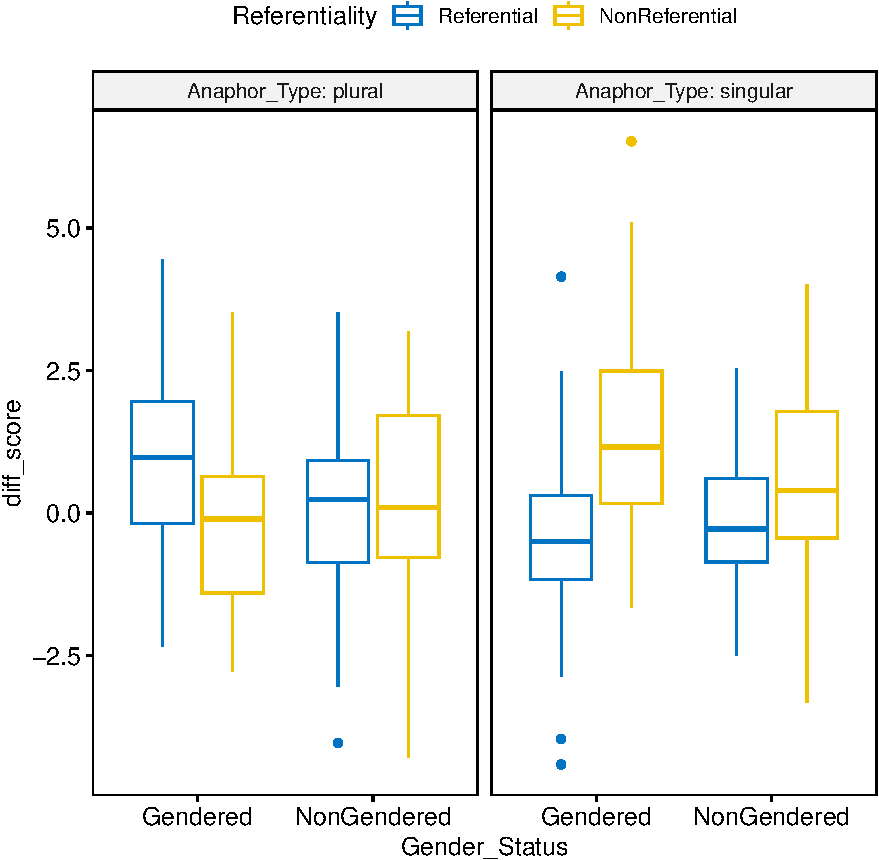
\includegraphics{prost_2022_n400_nref_by_group_files/figure-latex/unnamed-chunk-13-1.pdf}

\subsection{Interaction Plots: Group x Gender Status x Referentiality
Interaction:
Binary}\label{interaction-plots-group-x-gender-status-x-referentiality-interaction-binary}

~

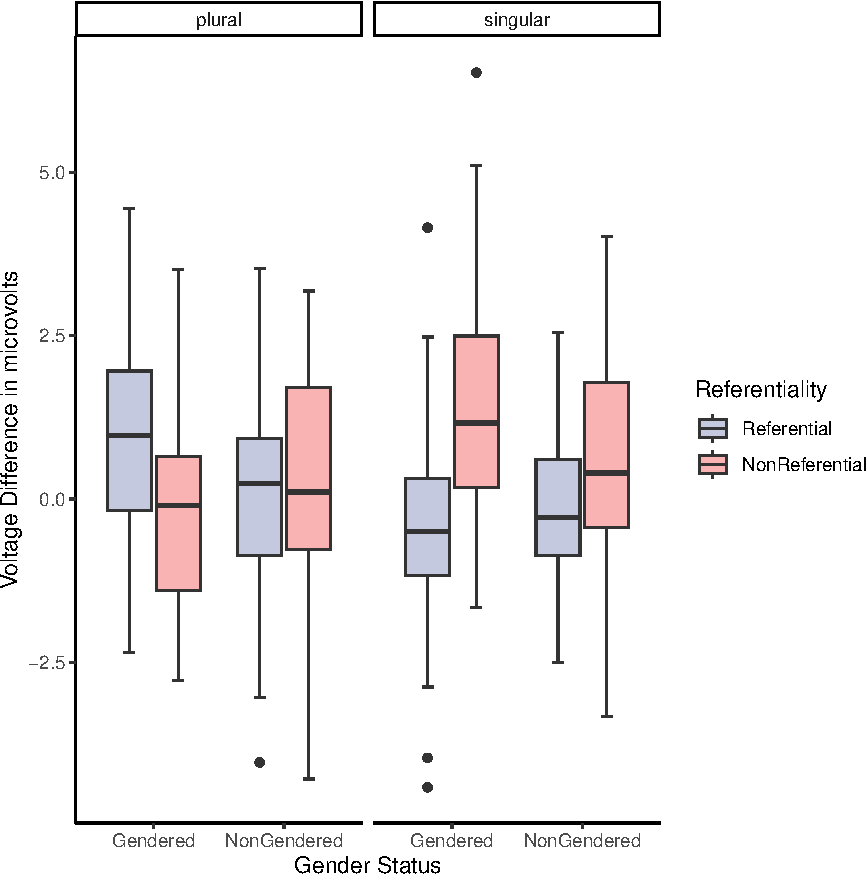
\includegraphics{prost_2022_n400_nref_by_group_files/figure-latex/unnamed-chunk-14-1.pdf}

\section{Visualization: Box plots with p-values
NONBINARY}\label{visualization-box-plots-with-p-values-nonbinary}

\subsubsection{\texorpdfstring{Compute simple simple main effects with
Bonferroni adjustment using \texttt{pwc()} function in the
\texttt{rstatix}}{Compute simple simple main effects with Bonferroni adjustment using pwc() function in the rstatix}}\label{compute-simple-simple-main-effects-with-bonferroni-adjustment-using-pwc-function-in-the-rstatix-1}

\begin{longtable}[]{@{}
  >{\raggedright\arraybackslash}p{(\columnwidth - 20\tabcolsep) * \real{0.1373}}
  >{\raggedright\arraybackslash}p{(\columnwidth - 20\tabcolsep) * \real{0.1078}}
  >{\raggedright\arraybackslash}p{(\columnwidth - 20\tabcolsep) * \real{0.1176}}
  >{\raggedright\arraybackslash}p{(\columnwidth - 20\tabcolsep) * \real{0.1471}}
  >{\raggedleft\arraybackslash}p{(\columnwidth - 20\tabcolsep) * \real{0.0294}}
  >{\raggedleft\arraybackslash}p{(\columnwidth - 20\tabcolsep) * \real{0.0294}}
  >{\raggedleft\arraybackslash}p{(\columnwidth - 20\tabcolsep) * \real{0.0980}}
  >{\raggedleft\arraybackslash}p{(\columnwidth - 20\tabcolsep) * \real{0.0294}}
  >{\raggedleft\arraybackslash}p{(\columnwidth - 20\tabcolsep) * \real{0.0882}}
  >{\raggedleft\arraybackslash}p{(\columnwidth - 20\tabcolsep) * \real{0.0882}}
  >{\raggedright\arraybackslash}p{(\columnwidth - 20\tabcolsep) * \real{0.1275}}@{}}
\toprule\noalign{}
\begin{minipage}[b]{\linewidth}\raggedright
Gender\_Status
\end{minipage} & \begin{minipage}[b]{\linewidth}\raggedright
.y.
\end{minipage} & \begin{minipage}[b]{\linewidth}\raggedright
group1
\end{minipage} & \begin{minipage}[b]{\linewidth}\raggedright
group2
\end{minipage} & \begin{minipage}[b]{\linewidth}\raggedleft
n1
\end{minipage} & \begin{minipage}[b]{\linewidth}\raggedleft
n2
\end{minipage} & \begin{minipage}[b]{\linewidth}\raggedleft
statistic
\end{minipage} & \begin{minipage}[b]{\linewidth}\raggedleft
df
\end{minipage} & \begin{minipage}[b]{\linewidth}\raggedleft
p
\end{minipage} & \begin{minipage}[b]{\linewidth}\raggedleft
p.adj
\end{minipage} & \begin{minipage}[b]{\linewidth}\raggedright
p.adj.signif
\end{minipage} \\
\midrule\noalign{}
\endhead
\bottomrule\noalign{}
\endlastfoot
Gendered & diff\_score & Referential & NonReferential & 90 & 90 &
-1.142697 & 89 & 2.56e-01 & 2.56e-01 & ns \\
NonGendered & diff\_score & Referential & NonReferential & 90 & 90 &
-5.201870 & 89 & 1.30e-06 & 1.30e-06 & **** \\
\end{longtable}

\includegraphics{prost_2022_n400_nref_by_group_files/figure-latex/unnamed-chunk-16-1.pdf}

\subsection{Interaction Plots: Group x Gender Status x Referentiality
NonBinary}\label{interaction-plots-group-x-gender-status-x-referentiality-nonbinary}

~

\includegraphics{prost_2022_n400_nref_by_group_files/figure-latex/unnamed-chunk-17-1.pdf}

\section{Post-hoc tests for Analysis 1: GROUP x ANTERIORITY
interaction}\label{post-hoc-tests-for-analysis-1-group-x-anteriority-interaction}

The following chunk runs post-hoc tests for the 2-way
\textbf{\emph{``Group x Anteriority''}} Interaction

\begin{Shaded}
\begin{Highlighting}[]
\CommentTok{\# Binary vs Non{-}Binary Frontal}

\FunctionTok{pander}\NormalTok{(}\FunctionTok{t.test}\NormalTok{(diff\_score }\SpecialCharTok{\textasciitilde{}}\NormalTok{ Group}
\NormalTok{       ,dplyr}\SpecialCharTok{::}\FunctionTok{filter}\NormalTok{(prost\_2024\_singular, (Anteriority }\SpecialCharTok{==} \StringTok{"Frontal"}\NormalTok{))))}
\end{Highlighting}
\end{Shaded}

\begin{longtable}[]{@{}
  >{\centering\arraybackslash}p{(\columnwidth - 8\tabcolsep) * \real{0.2048}}
  >{\centering\arraybackslash}p{(\columnwidth - 8\tabcolsep) * \real{0.0723}}
  >{\centering\arraybackslash}p{(\columnwidth - 8\tabcolsep) * \real{0.1205}}
  >{\centering\arraybackslash}p{(\columnwidth - 8\tabcolsep) * \real{0.3012}}
  >{\centering\arraybackslash}p{(\columnwidth - 8\tabcolsep) * \real{0.3012}}@{}}
\caption{Welch Two Sample t-test: \texttt{diff\_score} by \texttt{Group}
(continued below)}\tabularnewline
\toprule\noalign{}
\begin{minipage}[b]{\linewidth}\centering
Test statistic
\end{minipage} & \begin{minipage}[b]{\linewidth}\centering
df
\end{minipage} & \begin{minipage}[b]{\linewidth}\centering
P value
\end{minipage} & \begin{minipage}[b]{\linewidth}\centering
Alternative hypothesis
\end{minipage} & \begin{minipage}[b]{\linewidth}\centering
mean in group Binary
\end{minipage} \\
\midrule\noalign{}
\endfirsthead
\toprule\noalign{}
\begin{minipage}[b]{\linewidth}\centering
Test statistic
\end{minipage} & \begin{minipage}[b]{\linewidth}\centering
df
\end{minipage} & \begin{minipage}[b]{\linewidth}\centering
P value
\end{minipage} & \begin{minipage}[b]{\linewidth}\centering
Alternative hypothesis
\end{minipage} & \begin{minipage}[b]{\linewidth}\centering
mean in group Binary
\end{minipage} \\
\midrule\noalign{}
\endhead
\bottomrule\noalign{}
\endlastfoot
0.5115 & 150 & 0.6097 & two.sided & -0.12 \\
\end{longtable}

\begin{longtable}[]{@{}
  >{\centering\arraybackslash}p{(\columnwidth - 0\tabcolsep) * \real{0.3611}}@{}}
\toprule\noalign{}
\begin{minipage}[b]{\linewidth}\centering
mean in group NonBinary
\end{minipage} \\
\midrule\noalign{}
\endhead
\bottomrule\noalign{}
\endlastfoot
-0.3102 \\
\end{longtable}

\begin{Shaded}
\begin{Highlighting}[]
\CommentTok{\# Binary vs Non{-}Binary Fronto{-}Central}

\FunctionTok{pander}\NormalTok{(}\FunctionTok{t.test}\NormalTok{(diff\_score }\SpecialCharTok{\textasciitilde{}}\NormalTok{ Group}
\NormalTok{       ,dplyr}\SpecialCharTok{::}\FunctionTok{filter}\NormalTok{(prost\_2024\_singular, (Anteriority }\SpecialCharTok{==} \StringTok{"FrontoCentral"}\NormalTok{))))}
\end{Highlighting}
\end{Shaded}

\begin{longtable}[]{@{}
  >{\centering\arraybackslash}p{(\columnwidth - 6\tabcolsep) * \real{0.2361}}
  >{\centering\arraybackslash}p{(\columnwidth - 6\tabcolsep) * \real{0.1111}}
  >{\centering\arraybackslash}p{(\columnwidth - 6\tabcolsep) * \real{0.1389}}
  >{\centering\arraybackslash}p{(\columnwidth - 6\tabcolsep) * \real{0.3472}}@{}}
\caption{Welch Two Sample t-test: \texttt{diff\_score} by \texttt{Group}
(continued below)}\tabularnewline
\toprule\noalign{}
\begin{minipage}[b]{\linewidth}\centering
Test statistic
\end{minipage} & \begin{minipage}[b]{\linewidth}\centering
df
\end{minipage} & \begin{minipage}[b]{\linewidth}\centering
P value
\end{minipage} & \begin{minipage}[b]{\linewidth}\centering
Alternative hypothesis
\end{minipage} \\
\midrule\noalign{}
\endfirsthead
\toprule\noalign{}
\begin{minipage}[b]{\linewidth}\centering
Test statistic
\end{minipage} & \begin{minipage}[b]{\linewidth}\centering
df
\end{minipage} & \begin{minipage}[b]{\linewidth}\centering
P value
\end{minipage} & \begin{minipage}[b]{\linewidth}\centering
Alternative hypothesis
\end{minipage} \\
\midrule\noalign{}
\endhead
\bottomrule\noalign{}
\endlastfoot
-0.1109 & 149.9 & 0.9119 & two.sided \\
\end{longtable}

\begin{longtable}[]{@{}
  >{\centering\arraybackslash}p{(\columnwidth - 2\tabcolsep) * \real{0.3194}}
  >{\centering\arraybackslash}p{(\columnwidth - 2\tabcolsep) * \real{0.3611}}@{}}
\toprule\noalign{}
\begin{minipage}[b]{\linewidth}\centering
mean in group Binary
\end{minipage} & \begin{minipage}[b]{\linewidth}\centering
mean in group NonBinary
\end{minipage} \\
\midrule\noalign{}
\endhead
\bottomrule\noalign{}
\endlastfoot
-0.2496 & -0.2145 \\
\end{longtable}

\begin{Shaded}
\begin{Highlighting}[]
\CommentTok{\# Binary vs Non{-}Binary Central}

\FunctionTok{pander}\NormalTok{(}\FunctionTok{t.test}\NormalTok{(diff\_score }\SpecialCharTok{\textasciitilde{}}\NormalTok{ Group}
\NormalTok{       ,dplyr}\SpecialCharTok{::}\FunctionTok{filter}\NormalTok{(prost\_2024\_singular, (Anteriority }\SpecialCharTok{==} \StringTok{"Central"}\NormalTok{))))}
\end{Highlighting}
\end{Shaded}

\begin{longtable}[]{@{}
  >{\centering\arraybackslash}p{(\columnwidth - 6\tabcolsep) * \real{0.2361}}
  >{\centering\arraybackslash}p{(\columnwidth - 6\tabcolsep) * \real{0.1111}}
  >{\centering\arraybackslash}p{(\columnwidth - 6\tabcolsep) * \real{0.1389}}
  >{\centering\arraybackslash}p{(\columnwidth - 6\tabcolsep) * \real{0.3472}}@{}}
\caption{Welch Two Sample t-test: \texttt{diff\_score} by \texttt{Group}
(continued below)}\tabularnewline
\toprule\noalign{}
\begin{minipage}[b]{\linewidth}\centering
Test statistic
\end{minipage} & \begin{minipage}[b]{\linewidth}\centering
df
\end{minipage} & \begin{minipage}[b]{\linewidth}\centering
P value
\end{minipage} & \begin{minipage}[b]{\linewidth}\centering
Alternative hypothesis
\end{minipage} \\
\midrule\noalign{}
\endfirsthead
\toprule\noalign{}
\begin{minipage}[b]{\linewidth}\centering
Test statistic
\end{minipage} & \begin{minipage}[b]{\linewidth}\centering
df
\end{minipage} & \begin{minipage}[b]{\linewidth}\centering
P value
\end{minipage} & \begin{minipage}[b]{\linewidth}\centering
Alternative hypothesis
\end{minipage} \\
\midrule\noalign{}
\endhead
\bottomrule\noalign{}
\endlastfoot
-1.359 & 149.7 & 0.1761 & two.sided \\
\end{longtable}

\begin{longtable}[]{@{}
  >{\centering\arraybackslash}p{(\columnwidth - 2\tabcolsep) * \real{0.3194}}
  >{\centering\arraybackslash}p{(\columnwidth - 2\tabcolsep) * \real{0.3611}}@{}}
\toprule\noalign{}
\begin{minipage}[b]{\linewidth}\centering
mean in group Binary
\end{minipage} & \begin{minipage}[b]{\linewidth}\centering
mean in group NonBinary
\end{minipage} \\
\midrule\noalign{}
\endhead
\bottomrule\noalign{}
\endlastfoot
-0.3873 & 0.01419 \\
\end{longtable}

\begin{Shaded}
\begin{Highlighting}[]
\CommentTok{\# Binary vs Non{-}Binary Centro{-}Parietal}

\FunctionTok{pander}\NormalTok{(}\FunctionTok{t.test}\NormalTok{(diff\_score }\SpecialCharTok{\textasciitilde{}}\NormalTok{ Group}
\NormalTok{       ,dplyr}\SpecialCharTok{::}\FunctionTok{filter}\NormalTok{(prost\_2024\_singular, (Anteriority }\SpecialCharTok{==} \StringTok{"CentroParietal"}\NormalTok{))))}
\end{Highlighting}
\end{Shaded}

\begin{longtable}[]{@{}
  >{\centering\arraybackslash}p{(\columnwidth - 6\tabcolsep) * \real{0.2361}}
  >{\centering\arraybackslash}p{(\columnwidth - 6\tabcolsep) * \real{0.1111}}
  >{\centering\arraybackslash}p{(\columnwidth - 6\tabcolsep) * \real{0.1389}}
  >{\centering\arraybackslash}p{(\columnwidth - 6\tabcolsep) * \real{0.3472}}@{}}
\caption{Welch Two Sample t-test: \texttt{diff\_score} by \texttt{Group}
(continued below)}\tabularnewline
\toprule\noalign{}
\begin{minipage}[b]{\linewidth}\centering
Test statistic
\end{minipage} & \begin{minipage}[b]{\linewidth}\centering
df
\end{minipage} & \begin{minipage}[b]{\linewidth}\centering
P value
\end{minipage} & \begin{minipage}[b]{\linewidth}\centering
Alternative hypothesis
\end{minipage} \\
\midrule\noalign{}
\endfirsthead
\toprule\noalign{}
\begin{minipage}[b]{\linewidth}\centering
Test statistic
\end{minipage} & \begin{minipage}[b]{\linewidth}\centering
df
\end{minipage} & \begin{minipage}[b]{\linewidth}\centering
P value
\end{minipage} & \begin{minipage}[b]{\linewidth}\centering
Alternative hypothesis
\end{minipage} \\
\midrule\noalign{}
\endhead
\bottomrule\noalign{}
\endlastfoot
-1.853 & 149.6 & 0.06587 & two.sided \\
\end{longtable}

\begin{longtable}[]{@{}
  >{\centering\arraybackslash}p{(\columnwidth - 2\tabcolsep) * \real{0.3194}}
  >{\centering\arraybackslash}p{(\columnwidth - 2\tabcolsep) * \real{0.3611}}@{}}
\toprule\noalign{}
\begin{minipage}[b]{\linewidth}\centering
mean in group Binary
\end{minipage} & \begin{minipage}[b]{\linewidth}\centering
mean in group NonBinary
\end{minipage} \\
\midrule\noalign{}
\endhead
\bottomrule\noalign{}
\endlastfoot
-0.3836 & 0.1546 \\
\end{longtable}

\begin{Shaded}
\begin{Highlighting}[]
\CommentTok{\# Binary vs Non{-}Binary Parietal}

\FunctionTok{pander}\NormalTok{(}\FunctionTok{t.test}\NormalTok{(diff\_score }\SpecialCharTok{\textasciitilde{}}\NormalTok{ Group}
\NormalTok{       ,dplyr}\SpecialCharTok{::}\FunctionTok{filter}\NormalTok{(prost\_2024\_singular, (Anteriority }\SpecialCharTok{==} \StringTok{"Parietal"}\NormalTok{))))}
\end{Highlighting}
\end{Shaded}

\begin{longtable}[]{@{}
  >{\centering\arraybackslash}p{(\columnwidth - 6\tabcolsep) * \real{0.2361}}
  >{\centering\arraybackslash}p{(\columnwidth - 6\tabcolsep) * \real{0.1111}}
  >{\centering\arraybackslash}p{(\columnwidth - 6\tabcolsep) * \real{0.1667}}
  >{\centering\arraybackslash}p{(\columnwidth - 6\tabcolsep) * \real{0.3472}}@{}}
\caption{Welch Two Sample t-test: \texttt{diff\_score} by \texttt{Group}
(continued below)}\tabularnewline
\toprule\noalign{}
\begin{minipage}[b]{\linewidth}\centering
Test statistic
\end{minipage} & \begin{minipage}[b]{\linewidth}\centering
df
\end{minipage} & \begin{minipage}[b]{\linewidth}\centering
P value
\end{minipage} & \begin{minipage}[b]{\linewidth}\centering
Alternative hypothesis
\end{minipage} \\
\midrule\noalign{}
\endfirsthead
\toprule\noalign{}
\begin{minipage}[b]{\linewidth}\centering
Test statistic
\end{minipage} & \begin{minipage}[b]{\linewidth}\centering
df
\end{minipage} & \begin{minipage}[b]{\linewidth}\centering
P value
\end{minipage} & \begin{minipage}[b]{\linewidth}\centering
Alternative hypothesis
\end{minipage} \\
\midrule\noalign{}
\endhead
\bottomrule\noalign{}
\endlastfoot
-2.229 & 149.3 & 0.02728 * & two.sided \\
\end{longtable}

\begin{longtable}[]{@{}
  >{\centering\arraybackslash}p{(\columnwidth - 2\tabcolsep) * \real{0.3194}}
  >{\centering\arraybackslash}p{(\columnwidth - 2\tabcolsep) * \real{0.3611}}@{}}
\toprule\noalign{}
\begin{minipage}[b]{\linewidth}\centering
mean in group Binary
\end{minipage} & \begin{minipage}[b]{\linewidth}\centering
mean in group NonBinary
\end{minipage} \\
\midrule\noalign{}
\endhead
\bottomrule\noalign{}
\endlastfoot
-0.279 & 0.3568 \\
\end{longtable}

\section{Visualization: Box plots with
p-values}\label{visualization-box-plots-with-p-values}

\subsubsection{\texorpdfstring{Compute simple simple main effects with
Bonferroni adjustment using \texttt{pwc()} function in the
\texttt{rstatix}}{Compute simple simple main effects with Bonferroni adjustment using pwc() function in the rstatix}}\label{compute-simple-simple-main-effects-with-bonferroni-adjustment-using-pwc-function-in-the-rstatix-2}

\begin{longtable}[]{@{}
  >{\raggedright\arraybackslash}p{(\columnwidth - 18\tabcolsep) * \real{0.1765}}
  >{\raggedright\arraybackslash}p{(\columnwidth - 18\tabcolsep) * \real{0.1294}}
  >{\raggedright\arraybackslash}p{(\columnwidth - 18\tabcolsep) * \real{0.0824}}
  >{\raggedright\arraybackslash}p{(\columnwidth - 18\tabcolsep) * \real{0.1176}}
  >{\raggedleft\arraybackslash}p{(\columnwidth - 18\tabcolsep) * \real{0.0353}}
  >{\raggedleft\arraybackslash}p{(\columnwidth - 18\tabcolsep) * \real{0.0353}}
  >{\raggedleft\arraybackslash}p{(\columnwidth - 18\tabcolsep) * \real{0.0824}}
  >{\raggedright\arraybackslash}p{(\columnwidth - 18\tabcolsep) * \real{0.1059}}
  >{\raggedleft\arraybackslash}p{(\columnwidth - 18\tabcolsep) * \real{0.0824}}
  >{\raggedright\arraybackslash}p{(\columnwidth - 18\tabcolsep) * \real{0.1529}}@{}}
\toprule\noalign{}
\begin{minipage}[b]{\linewidth}\raggedright
Anteriority
\end{minipage} & \begin{minipage}[b]{\linewidth}\raggedright
.y.
\end{minipage} & \begin{minipage}[b]{\linewidth}\raggedright
group1
\end{minipage} & \begin{minipage}[b]{\linewidth}\raggedright
group2
\end{minipage} & \begin{minipage}[b]{\linewidth}\raggedleft
n1
\end{minipage} & \begin{minipage}[b]{\linewidth}\raggedleft
n2
\end{minipage} & \begin{minipage}[b]{\linewidth}\raggedleft
p
\end{minipage} & \begin{minipage}[b]{\linewidth}\raggedright
p.signif
\end{minipage} & \begin{minipage}[b]{\linewidth}\raggedleft
p.adj
\end{minipage} & \begin{minipage}[b]{\linewidth}\raggedright
p.adj.signif
\end{minipage} \\
\midrule\noalign{}
\endhead
\bottomrule\noalign{}
\endlastfoot
Frontal & diff\_score & Binary & NonBinary & 80 & 72 & 0.6120 & ns &
0.6120 & ns \\
FrontoCentral & diff\_score & Binary & NonBinary & 80 & 72 & 0.9120 & ns
& 0.9120 & ns \\
Central & diff\_score & Binary & NonBinary & 80 & 72 & 0.1770 & ns &
0.1770 & ns \\
CentroParietal & diff\_score & Binary & NonBinary & 80 & 72 & 0.0666 &
ns & 0.0666 & ns \\
Parietal & diff\_score & Binary & NonBinary & 80 & 72 & 0.0276 & * &
0.0276 & * \\
\end{longtable}

\includegraphics{prost_2022_n400_nref_by_group_files/figure-latex/unnamed-chunk-20-1.pdf}

\subparagraph{Interaction Plot: Group x
Anteriority}\label{interaction-plot-group-x-anteriority}

~

\includegraphics{prost_2022_n400_nref_by_group_files/figure-latex/unnamed-chunk-21-1.pdf}

\includegraphics{prost_2022_n400_nref_by_group_files/figure-latex/unnamed-chunk-22-1.pdf}

\end{document}
